\section{Introduction}

%
% Thanks to Martha Field for discussion on adapting mammalian cells
% to synthetic media.
%
FBA (flux balance analysis) has become extremely popular, in part, due
to its simplicity in calculating reasonably accurate microbial fluxes
or growth rates (e.g.\ \citealt{Schuetz2012,Fong2004_sb2013}); for
many microbes, a simple synthetic environment where all chemical
species are known suffices to allow proliferation, giving fairly
complete constraints on model inputs. Additionally, it has been found
that their biological objectives can be largely expressed as linear
objectives of fluxes \citep{Schuetz2012}.  Neither of these
assumptions necessarily hold for mammalian cells growing \textit{in
  vitro} or \textit{in vivo}, and in particular the environment is far
more complex for mammalian cell cultures, which have to undergo
gradual metabolic adaptation via titration to grow on synthetic media
\citep{Pirkmajer2011}. In what follows we first discuss the MoMA
algorithm since it is heavily extended in order to allow us to use
expression data for the estimation of flux data.

% May eventually want to make this a conditional include section
% and include it earlier in dissertation.
%\subsection{MoMA: Minimization of Metabolic Adjustment}

The minimization of metabolic adjustment (MoMA) method
\citep{Segre2002}, which is framed as a constrained least-squares optimization
problem, is typically employed to calculate the flux vector of an
\textit{in silico} organism after a mutation by minimizing the distance
between the wild-type flux and the mutant flux. The biological
intuition is that the organism has not had time to adapt to the
restricted metabolic capacity and will maintain a similar flux to the
wild-type (WT) except where the perturbations due to the mutation
dictate necessary alterations in fluxes \citep{Shlomi2005}.

Suppose $\mathbf{a}$ is the WT flux vector obtained by an optimization
procedure such as FBA, empirical measurements, or a combination of
these. For an undetermined flux vector $\mathbf{v}$ in a model with
$N$ reactions the objective can be expressed as
\[ \textnormal{minimize}\ \sum\limits_{i=1}^N (v_i-a_i)^2 \] 
subject to the stoichiometric constraints $\mathbf{S v}\nolinebreak
=\nolinebreak \mathbf{0}$ where $\mathbf{v} = (v_1, \ldots,
v_N)^T$. The objective may be equivalently expressed in the canonical
quadratic programming (QP) vector form as
$\textnormal{min.\ }\ \frac{1}{2}\mathbf{v}^T \mathbf{v}\nolinebreak
-\nolinebreak \mathbf{a}^T \mathbf{v}$. This assumes that each $a_i$
is measured, but it is also possible and sometimes even more useful to
employ this objective when only a subset of the $a_i$ are measured (if
$a_i$ is not measured for some $i$, then we omit $(v_i-a_i)^2$ from
the objective). In metabolomics, for instance, it is always the case
in experiments with labeled isotope tracers that only a relatively
small subset of all fluxes are able to be estimated with metabolic
flux analysis (MFA; \citealt{Shestov2013}). Combining MoMA with MFA
provides a technique to potentially estimate other fluxes in the
network.  Constant bounds on fluxes are often present, such as
substrate uptake limits, or experimental $V_{\max}$ estimates, so we
write these as the constraints $\mathbf{v}_{lb}\nolinebreak
\preceq\nolinebreak \mathbf{v}\nolinebreak \preceq \mathbf{v}_{ub}$.

A variant of MoMA exists that minimizes the absolute value of the
difference between $a_i$ and $v_i$ for all known $a_i$. To our
knowledge, the following linear program is the simplest version of
linear MoMA, which assumes the existence of a constant flux vector
$\mathbf{a}$ and is expressed as the following linear program:

\begin{center}
\begin{tabular}{rl}
minimize & $\sum\limits_{i=1}^N d_i$  \\
subject to & $\mathbf{S v} = \mathbf{0}$ \\
 & $\mathbf{v}_{lb} \preceq \mathbf{v} \preceq \mathbf{v}_{ub}$ \\
$\forall i:$ & $-d_i \le v_i-a_i \le d_i$ \\
 & $d_i \ge 0$
\end{tabular}
\end{center}

The $d_i$ are just the distances from \textit{a priori} fluxes to
their corresponding fitted fluxes.  Linear MoMA has the advantage that
it is not biased towards penalizing large magnitude fluxes or
under-penalizing fluxes that are less than one
\citep{Boyd2004,Shlomi2005}. Additionally, linear programs are often
amenable to more alterations that maintain convexity than a quadratic
program.

\section{Methods}

In order to develop software that is easy to use and shares a popular API,
our software is largely implemented in MATLAB using the COBRA
Toolbox \citep{Hyduke2011}. The first algorithm in the technique
has been implemented in ATS, a C-code generating language with rich
safety features, in order to attain good time-efficiency without sacrificing
safety and stability \citep{ATStypes03}. The only expensive operations in the
MATLAB code are external calls to a linear program (LP) solver,
so the efficiency in this case depends on the solver and the metabolic
model in a complicated manner due to diverse algorithms and
implementions as well as sensitivity to the model parameters
\citep{Mittelmann2013,Todd2002}. We discuss performance statistics for
several models below using a state-of-the-art solver \ref{Table XX,
  Supp Note XX}. Before comparing this approach to related methods, we
describe our rationale and algorithms.

If we wish to apply MoMA to expression data rather than flux data, the
original MoMA objective must be altered in several ways. Scaling of
expression values must be addressed so they can be comparable to
fluxes in the minimization. Also, expression data has no
directionality, necessitating reaction direction assignment in order
to compare enzyme complex copy number and flux directly in the
optimization problem \citep{Lee2012}.

Most genome-scale models have attached Boolean (\textit{sans}
negation) gene rules to aid in determining whether or not a gene
deletion will
completely disable a reaction. These are typically called GPR
(gene-protein-reaction) rules and are a requirement for FALCON; their
validity, like the stoichiometric matrix, will undoubtedly be
important for generating accurate predictions. Also important are the
assumptions and limitations for the process of mapping expression data
to complexes so that a scaled enzyme complex copy number (hereafter
referred to as complex abundance) can be estimated. We address these
in the next section and have attached a flow chart to illustrate the
overall process of mapping expression of individual genes to enzyme
complexes (Figure~\ref{ECCN_flowchart}). We develop an algorithm for
this step---finding the minimum disjunction---where complex abundance
is estimated efficiently and as accurately as possible given the
assumptions (due primarily to limitations in data quality; \suppOrApp
Section~\ref{sec:complexation}).

\vspace{5 mm} 
\begin{figure}
\begin{center}
\begin{tikzpicture}%[scale=0.8, node distance = 1cm, auto]
    % Place nodes
    \node [block] (start) {start}; 
    \node [iogram, below of=start, left of=start] (exp) {Gene: 
      $\mu$,~$\sigma^2$}; 
    \node [iogram, below of=start, right of=start] (rules) {Reaction:
      Gene Rule}; 
    \node [block, below of=rules] (parse) {Parse Rule}; 
    \node [block, below of=parse, left of=parse, xshift=-0.5cm]
      (mindisj) {Find minimum disjunction};
    \node [iogram, below of=mindisj] (expstd)
          {Reaction\\(enzyme~complex): $\mu$,~$\sigma^2$};
    % Draw edges
    \path [line] (start) -- (exp);
    \path [line] (start) -- (rules);
    \path [line] (rules) -- (parse);
    \path [line] (exp.south) -- (mindisj);
    \path [line] (parse) -- (mindisj);
    \path [line] (mindisj) -- (expstd);
\end{tikzpicture}
\end{center}
\caption{Flowchart illustrating the process of estimating enzyme
  complex abundance. First, for each gene in the model with
  available expression data, the mean and (if available) variance or
  some other measure of uncertainty are read in. Gene rules (also
  called GPR rules) are also read in for each enzymatic reaction. The
  reaction rules are parsed and the minimum disjunction algorithm
  (Algorithm~\ref{alg:ReductionToCNF}) is applied, making use of the
  gene's mean expression. Finally, the estimated and unitless enzyme
  complex copy number and variance are output for each enzymatic
  reaction.}
\label{ECCN_flowchart}
\end{figure}

\subsection{A Formalism for Enzyme Complex Formation}

Given the abundance of genome-scale expression datasets available,
either as microarray or more recently RNA-Seq, it could be useful to
actually gauge the number of enzyme complexes present in a cell. This
isn't much of an issue for the simplest case where a reaction is
catalyzed by only one polypeptide, and that polypeptide does not
catalyze any other reactions.  Frequently the situation is not so
simple (e.g.\ Figure~\ref{fig:2F43}), so a model of enzyme complex
formation is called for.  We formalize such a model for enzyme complex
formation based on GPR (gene-protein-reaction) rules that are
frequently available in genome-scale annotations. For better curated
models, the approach described immediately finds use for understanding
metabolism, as well as being a scaffold to find problems for existing
GPRs, and more broadly the GPR formalism itself.

\subsubsection{Assumptions for Enzyme Complex Formation}
\emph{Assumption~\ref{asm:expcorr}.}  The first assumption that we
need in order to guarantee an accurate estimate of (relative) enzyme
complex copy number are accurate measurements of their component
subunits. Unfortunately, this is currently not possible, and we almost
always must make do with mRNA measurements, which may even have some
degree of inaccuracy in measuring the mRNA copy number. What has been
seen is that Spearman's $\rho = 0.6$ for correlation between RNA-Seq
and protein inensity in datasets from HeLa cells
\citep{Nagaraj2011}. This implies that much can likely still be
gleamed from analyzing RNA-Seq data, but, an appropriate degree of
caution must be used in interpreting results based on RNA-Seq data. By
incorporating more information, such as metabolic constaints, we hope
to obviate some of the error in estimating protein intensity from
RNA-Seq data.

\emph{Assumption~\ref{asm:isozyme}.}  In order to quantify enzyme
complex formation, the notion of an enzyme complex should be
formalized.  A protein complex typically refers to two or more
physically associated polypeptide chains, which is sometimes called a
quaternary structure. Since we are not exclusively dealing with
multiprotein complexes, we refer to an enzyme complex as being one or
more polypeptide chains that act together to carry out metabolic
catalysis. Also, to simply our English, we also include the notion of
isozymes--different proteins that catalyze the same reaction--in our
notion of enzyme complex. Isozymes may arise by having one or more
differing protein isoforms, and even though these isoforms may not be
present in the same complex at the same moment, we consider them to be
part of the enzyme complex since one could be substituted for the
other.

As an example, take the $F_1$ subcomplex of ATP Synthase (Figure
~\ref{fig:2F43}), which is composed of seven protein subunits
(distinguised by color, left). On the right-hand side we see different
isoforms depicted as different colors.  Error in expression data
aside, instead of considering the copy numbers with multiplicity and
dividing their expression values by their multiplicity, it may be
easier to simply note that the axle peptide (shown in red in the
center of the complex) only has one copy in the complex, so its
expression should be an overall good estimation of the $F_1$
subcomplex copy number. This reasoning will be useful later in
considering why GPRs may be largely adequate for estimating the
abundance of most enzyme complexes.

\begin{figure*}%[H]
\label{fig:2F43}
\centering
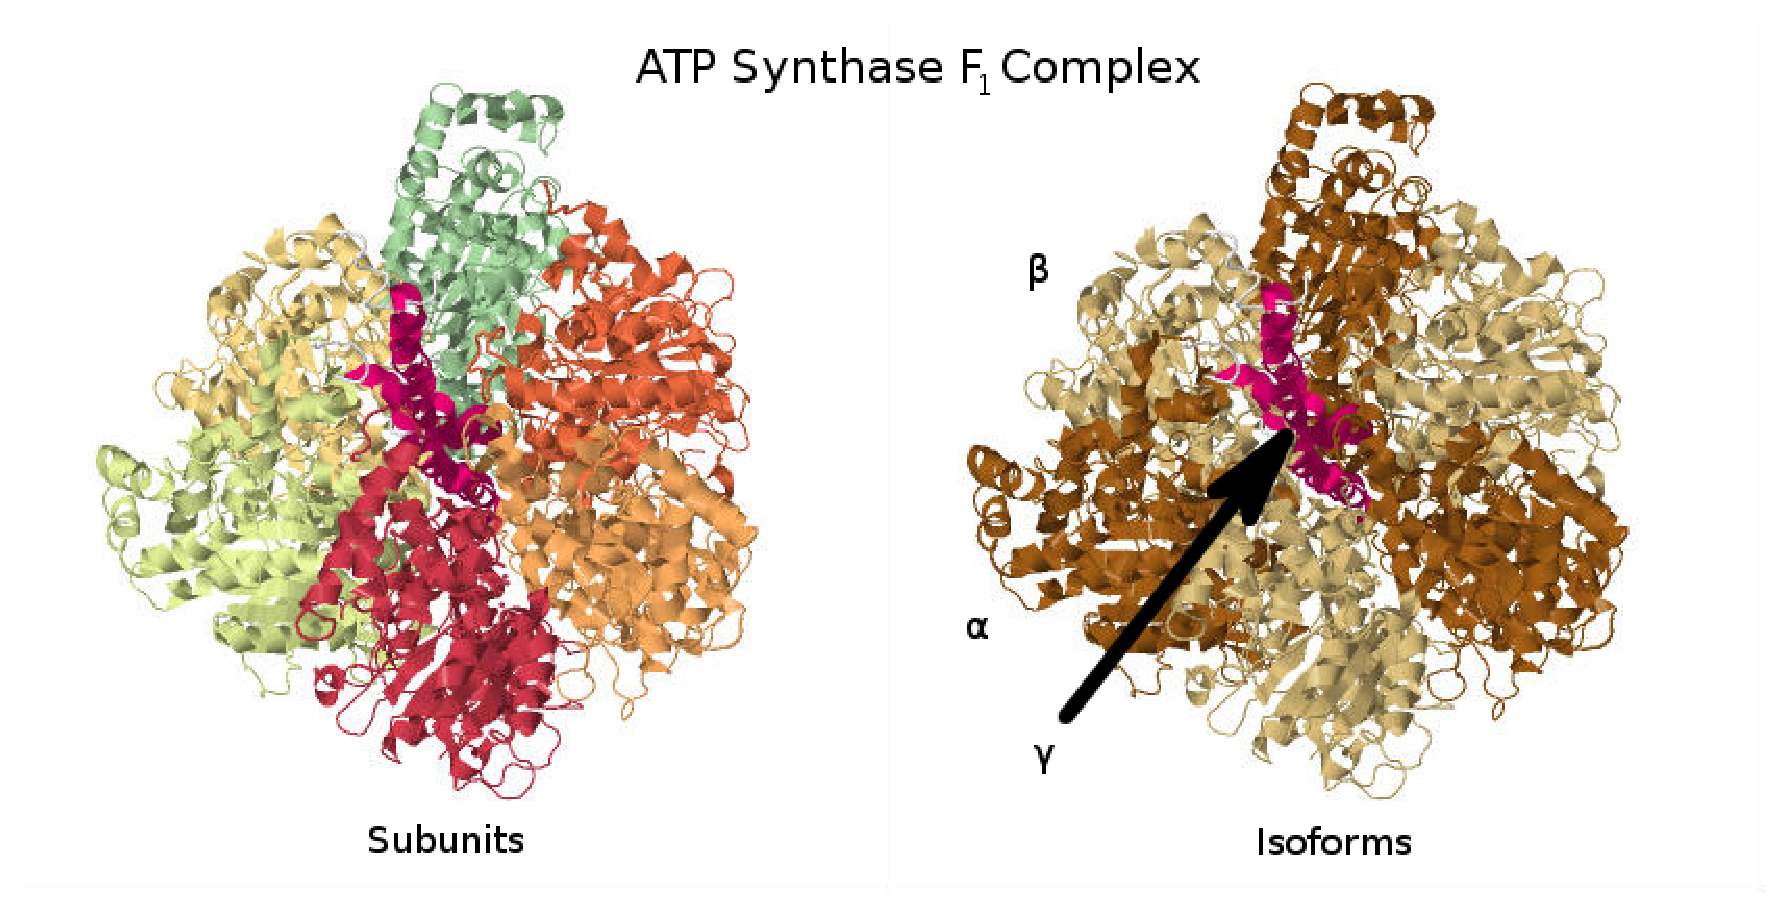
\includegraphics[clip=true,trim=0cm 0cm 0cm 0cm, width=12cm]{2F43}
\caption{Illustration of the $F_1$ part of the ATP Synthase complex
  (PDB ID 1E79; \citealt{Gibbons2000,Bernstein1978,Gezelter}).
  This illustration demonstrates both how an enzyme complex may be
  constituted by multiple subunits (left), and how some of those
  subunits may be products of the same gene and have differing
  stoichiometries within the complex (right).}
\end{figure*}

\emph{Assumption~\ref{asm:hierarchy}.}
The original expression to complex abundance mapping procedure
performed a direct evaluation of gene rule expression
values---replacing gene names with their expression values, ANDs with
minimums, and ORs with sums, without altering the logical expression
of the GPR rule in any way---can lead to problems in some
cases~\citep{Lee2012}. We illustrate this below; lower case letters
denote expression level (i.e.\ copy number of mRNA) of their
corresponding upper case letter, which denotes the gene name. The
$r_i$ are different reaction rules and the $e_i$ are the corresponding
estimated complex expression levels.

We need some way to guarantee that we don’t count anything twice or
more across disjunctions: 
\begin{AlgFloat}[H]
{\setlength{\tabcolsep}{.16667em}
\begin{tabular}{cccccccc}
& $r_1$ & := & [A and B] or [A and C] & $\rightarrow$ & $e_1$  &=& $\min(a,b$) + $\min(a,c$) \\ 
& $r_2$ & := & [A and (B or C)]       & $\rightarrow$ & $e_2$  &=&  $\min(a, b + c$) 
\end{tabular} 
}
\end{AlgFloat}
%Really we should be testing for number of text columns:
%\ifthenelse{\boolean{thesisStyle}}{\ruleEx1}{\hspace*{-4em}{\ruleEx1}} 

Supposing A is the minimum, then if we just evaluate $r_1$ directly (a
rule in disjunctive normal form, or DNF), A will be counted twice.

Another possibility is divvying up expression for a rule in DNF. For
instance, in $r_1$ above, we could evaluate it as $e_1$ =
min($\frac{a}{2},b$) + min($\frac{a}{2},c$) to account for the
repeated use of $a$. However, other potential issues aside, we can see
that this can cause problems rather quickly. For instance, suppose $b
= a$ and $c = 0$; then min($a$,$b+c$) $=b=a$ appears to be correct,
not min($\frac{a}{2},b$) + min($\frac{a}{2},c$) = $\frac{a}{2} + 0$.

The modeling of enzyme complex copy number can be tackled by using
nested sets of subcomplexes; each enzyme complex consists of multiple
subcomplexes, unlesss it is only a single protein or family of protein
isozymes.  These subcomplexes are required for the enzyme complex to
function (AND relationships), and can be thought of as the division of
the complex in to distinct units that each have some necessary
function for the complex, with the exception that we do not keep track
of the multiplicity of subcomplexes within a complex since this
information is, in the current state of affairs, not always known.
However, there may be alternative versions of each functional set
(given by OR relationships). Eventually, this nested embedding
terminates with a single protein or set of peptide isoforms
(e.g.\ isozymes).  In the case of ATP Synthase, one of its functional
sets is represented by the $F_1$ subcomplex. The $F_1$ subcomplex
itself can be viewed as having two immediate subcomplexes: the single
$\gamma$ (axle) subunit and three identical subcomplexes each made of
an $\alpha$ and $\beta$ subunit. Each $\alpha\beta$ pair works
together to bind ADP and catalyze the reaction \citep{Oster2003}. The
$\alpha\beta$ subcomplex itself then has two subcomplexes composed of
just an $\alpha$ subunit on the one hand and the $\beta$ subunit on
the other.  It is obvious that one of these base-level functional
subcomplexes (in this example, either $\gamma$ or $\alpha\beta$) will
be in most limited supply, and that it will best represent the overall
enzyme complex copy number (discounting the issues of multiplicity for
$\alpha\beta$, discussed above).

%
% Consider adding this as a Theorem/Proof:
%

The hierarhical structure just described, when written out in Boolean,
will give a rule in CNF (conjunctive normal form). This is because all
relations are ANDs (conjunctions), except possibly at the inner-most
subcomplexes that have alternative isoforms, which are expressed as
ORs (disjunctions). Since GPR rules alone only specify the
requirements for enzyme complex formation, we will see that not all
forms of boolean rules are equally useful in evaluating the enzyme
complex copy number, but we have established the assumptions in
Table~\ref{ECAssume} and an alternative and logically equivalent rule
\citep{Russell2009} under which we can estimate enzyme complex copy
number.


\def \ECAssumeCap {Assumptions in GPR-based Enzyme Complex Formation}
\label{ECAssume}
\ifthenelse{\boolean{thesisStyle}}{
  \begin{tabular}{| p{\textwidth} |}
  \hline
  \textbf{Table ~\ref{ECAssume}. \ECAssumeCap} \\
  \hline
  % I put this in to a separate file because formatting the table in different ways
% is difficult; it may even be better to have multiple versions of this table
% for different documents, but hopefully we can avoid such code duplication.

%Internal part of the table:

\begin{enumerate}
% This is really not related to GPR rules: 
%\ifthenelse{\boolean{thesisStyle}}{\item} {} \label{asm:mm}
%Fluxes in general strive to operate near the $V_{max}$ of the
%reaction, which is proportional to enzyme complex abundance.
\item \label{asm:expcorr}
Expression values are highly correlated with the copy numbers of their
corresponding peptide isoforms.
\item \label{asm:isozyme} 
Protein isoforms contributing to isozymes are considered part of the
same enzyme complex.
\item \label{asm:hierarchy}
Any enzyme complex can be described as a hierarchical subset of
(possibly redundant) subcomplexes; redundant subcomplexes, as
elaborated in (\ref{asm:nostoich}), are not currently modeled.
\item \label{asm:nostoich} 
Assume one copy of peptide per complex; exact isoform stoichiometry
is not considered.
\item \label{asm:sharing} 
With the exception of complexes having identical rules (i.e. the same
complex listed for different reactions), each copy of a peptide
is available for all complexes in the model.
\item \label{asm:active_site}
There is only one active site per enzyme complex.
\item \label{asm:enzyme_sensitivity} 
We assume that different pathways have similar flux sensitivities
with respect to their enzyme abundances.
\item \label{asm:holo} 
If a particular subcomplex can be catalyzed by A and it can also be
catalyzed by A and B (e.g. B acts as a regulatory unit, as in
holoenzymes), this just simplifies to A once expression values are
substituted in. Similarly, allosteric regulation is not
modeled. Relatedly, there are no NOT operations in GPR rules (just ANDs
and ORs).
\item \label{asm:chap} 
Enzyme complexes form without the assistance of protein chaperones and
formation is not coupled to other reactions.
\item \label{asm:posttrans}
Post-translational modifications do not affect complex formation.
\item \label{asm:rate} 
Rate of formation and degradation of complexes doesn't play a role,
since we assume steady-state. 
\end{enumerate}

  \\ \hline
  \end{tabular}

} {
  % For Bioinformatics:
  \begin{table*}[!t]
  \processtable{\ECAssumeCap \label{ECAssume}}{
  \begin{tabular}{| p{\textwidth} |}
  \hline
  % I put this in to a separate file because formatting the table in different ways
% is difficult; it may even be better to have multiple versions of this table
% for different documents, but hopefully we can avoid such code duplication.

%Internal part of the table:

\begin{enumerate}
% This is really not related to GPR rules: 
%\ifthenelse{\boolean{thesisStyle}}{\item} {} \label{asm:mm}
%Fluxes in general strive to operate near the $V_{max}$ of the
%reaction, which is proportional to enzyme complex abundance.
\item \label{asm:expcorr}
Expression values are highly correlated with the copy numbers of their
corresponding peptide isoforms.
\item \label{asm:isozyme} 
Protein isoforms contributing to isozymes are considered part of the
same enzyme complex.
\item \label{asm:hierarchy}
Any enzyme complex can be described as a hierarchical subset of
(possibly redundant) subcomplexes; redundant subcomplexes, as
elaborated in (\ref{asm:nostoich}), are not currently modeled.
\item \label{asm:nostoich} 
Assume one copy of peptide per complex; exact isoform stoichiometry
is not considered.
\item \label{asm:sharing} 
With the exception of complexes having identical rules (i.e. the same
complex listed for different reactions), each copy of a peptide
is available for all complexes in the model.
\item \label{asm:active_site}
There is only one active site per enzyme complex.
\item \label{asm:enzyme_sensitivity} 
We assume that different pathways have similar flux sensitivities
with respect to their enzyme abundances.
\item \label{asm:holo} 
If a particular subcomplex can be catalyzed by A and it can also be
catalyzed by A and B (e.g. B acts as a regulatory unit, as in
holoenzymes), this just simplifies to A once expression values are
substituted in. Similarly, allosteric regulation is not
modeled. Relatedly, there are no NOT operations in GPR rules (just ANDs
and ORs).
\item \label{asm:chap} 
Enzyme complexes form without the assistance of protein chaperones and
formation is not coupled to other reactions.
\item \label{asm:posttrans}
Post-translational modifications do not affect complex formation.
\item \label{asm:rate} 
Rate of formation and degradation of complexes doesn't play a role,
since we assume steady-state. 
\end{enumerate}

  \\ \hline
  \end{tabular}
  }
  {} % caption
  \end{table*}
}

There is no guarantee that a GPR rule has been written down with this
hierarchical structure in mind, though it is likely the case much of
the time as it is a natural way to model complexes.  However, any GPR
rule can be interpreted in the context of this hierarchical view due
to the existence of a logically equivlaent CNF rule for any non-CNF
rule, and it is obvious that logical equivalence is all that is
required to check for enzyme complex formation when exact isoform
stoichiometry is unknown.  As an example, we consider another common
formulation for GPRs, and a way to think about enzyme
structure---disjunctive normal form (DNF).  A DNF rule is a
disjunctive list of conjunctions of peptide isoforms, where each
conjunction is some variation of the enzyme complex due to
substituting in different isoforms for some of the required
subunits. A rule with a more complicated structure and compatible
isoforms across subcomplexes may be written more succinctinly in CNF,
whereas a rule with only very few alternatives derived from isoform
variants may be reprsented clearly with DNF.  In rare cases, it is
possible that a GPR rule is written in neither DNF or CNF, perhaps
because neither of these two alternatives above are stricly the case,
and some other rule is more succinct.

\emph{Assumptions~\ref{asm:nostoich},~\ref{asm:sharing}~and~\ref{asm:active_site}.}
One active site per enzyme complex implies a single complex can only
catalyze one reaction at a time. Multimeric complexes with one active
site per identical subunit would be considered as one enzyme complex
per subunit in this model.  Note that it is possible for an enzyme
complex to catalyze different reactions. In fact, some transporter
complexes can transfer many different metabolites \hl{across a lipid
  bilayer---up to}. Another example is the ligation or hydrolysis of
nucleotide, fatty acid, or peptide chains, where chains of different
length may all be substrates or products of the same enzyme
complex. While we do not explicitly consider these in
Algorithm~\ref{alg:ReductionToCNF}, these redundancies are taken into
account subsequently in Algorithm~\ref{alg:FALCON}.

What is currently not considered in our process is that some peptide
isoforms may find use in completely different complexes, and in some
cases, individual peptides may have multiple active sites; in the
first case, we assume an unrealistic case of superposition where the
isoform can simultaneously function in more than one complex. The
primary reason we have not tackled this problem is because exact
subunit stoichiometry of most enzyme complexes is not accurately
known, but an increasing abundance of data on BRENDA
\citep{Schomburg2013} gives some hope to this problem. A recent
\textit{E. coli} ME-model \citep{O'Brien2013} incorporates putative
enzyme complex stoichiometry into GPRs. For the second point, there
are a few enzymes where a single polpeptide may have multiple active
sites (e.g.\ fatty acid synthase), and this is not currently taken into
account in our model.

\emph{Assumption~\ref{asm:holo}.}
We do not make any special assumptions requiring symmetry of an
isoform within a complex. For instance, the example in
assumption~\ref{asm:holo} shows how you might have one subcomponent
composed of a single isoform, and another subcomponent composed of
that gene in addition to another isoform. In this case, it is simply
reduced to being the first gene only that is required, since clearly
the second is strictly optional. That isn't to say that the second
gene may not have some effect, such as (potentially) aiding in
structural ability or altering the catalytic rate, but it should have
no bearing on the formation of a functional catalytic
complex. Holoenzymes---enzymes with metabolic cofactors or protein
subunits that have a regulatory function for the complex---would
likely be the only situation where this type of rule might need to be
considered in more detail. But in the absence of detailed kinetic
information, this consideration not be useful, much like allosteric
regulation.

\emph{Assumptions~\ref{asm:chap}~and~\ref{asm:rate}.}
Due to the quickness, stability, and energetic favorability of enzyme
complex formation, the absence of chaperones or coupled metabolic
reactions required for complex formation may be reasonable
assumptions, but further research is warranted \citep{Karr2012}.
Additionally, as in metabolism, we assume a steady state for complex
formation, so that rate laws regarding complex formation aren't
needed. However, further research may be warranted to investigate the
use of a penalty for complex levels based on mass action and
protein-docking information. Requisite to this would be addressing
assumption~\ref{asm:nostoich}. It would be surprising (but not
impossible) if such a penalty were very larege due to the cost this
would imply for many of the large and important enzyme complexes
present in all organisms \citep{Nelson2008}.

\subsection{The min-disjunction algorithm estimates \\enzyme complex abundance}

In the previous section, we showed that converting a rule to CNF is a
sound method to aid in the estimation of enzyme complex copy number.
However, attempting to symbolically convert some rules in yeast models and
many rules in human models to CNF is computationally intractable due
to an exponential increase in memory \citep{Russell2009}. Therefore,
we use a reduction rule that makes use of expression data, outlined
below.  Note that the $AND$ and $OR$ notation is used to illustrate a
data structure that represents a set of literals that are
conjunctively or disjunctively joined together. The algorithm can be
described as follows:

\begin{AlgFloat}[H]
\begin{Algorithm}[min disjunction]
\label{alg:ReductionToCNF}
\begin{algorithmic}
\ifthenelse{\boolean{thesisStyle}}{\singlespacing}{}
~
\REQUIRE $g_i~s.t.~i \in{1, ..., m}$ are genes. 
\REQUIRE $x_i~s.t.~i \in{1, ..., n}$ are expressions in Boolean logic.
\WHILE{$rule \neq AND(o_1,...,o_p)$ where each $o_i$ has the form: $OR(...,g_j,...)~s.t.~j \leq m$}
  \STATE $\mathbf{1}$: check for sequence of ANDs of literals (genes)\\ 
    \hspace{4.8 mm} $\rightarrow$ reduce to gene with minimum expression 
  \STATE $\mathbf{2}$: Distribute ORs over ANDs, e.g.: $(x_1 \land x_2) \lor (x_3 \land x_4)$ \\ 
    \hspace{4.8 mm} $\rightarrow (x_1 \lor x_3) \land (x_1 \lor x_4) \land (x_2 \lor x_3) \land (x_2 \lor x_4)$
  \STATE $\mathbf{3}$: Change adjacent gene arguments to sets, e.g: \\
    \hspace{4.8 mm} $g_1 \land g_2 \rightarrow AND(g_1,g_2)$;  \\
    \hspace{4.8 mm} $g_1 \land AND(g_2,g_3) \rightarrow AND(g_1,g_2,g_3)$ 
\ENDWHILE
\ENSURE $o_{\min}$ where $o_{\min}$ has the form: $OR(g_1,...,g_m)$
\end{algorithmic} 
\end{Algorithm}
\end{AlgFloat}

The third step greatly simplifies numeric manipulations and checking
for the terminating condition. Please see the
\suppOrApp (Section~\ref{sec:code}) for the related core algorithmic 
code. This algorithm returns the minimum disjunction because at
each iteration, we select the literal with smallest value in a
conjunction and remove all other literals in the conjuction;
distributing ORs over ANDs and subsequently evaluating the associated
expression values will not change which disjunction attains the
minimum value. A slightly more detailed proof is given in the
\suppOrApp~(\ref{thm:ReductionToCNF}).

\subsection{Formulation with Automatic Normalization and Fast Direction Assignment}

Prior work that served as an inspiration for this method used Flux
Variability Analysis (FVA) to determine reaction direction
\citep{Lee2012}. Briefly, this involves two FBA simulations per
reaction catalyzed by an enzyme, and as the algorithm is iterative,
this global procedure may be run several times before converging to a
flux vector.  We removed FVA to mitigate some
of the cost, and instead assign flux direction in batch; while it is
possible that the objective value may decrease using this approach,
this is not an issue since the objetive function increases to include
more irreversible fluxes at each iteration, and the objective value of
a function with more fluxes should supersede the importance of one
with fewer fluxes.
 
To make working with irreversible fluxes simpler, we convert the model
to an irreversible model, where each reversible flux $v_j$ in the
original model is split into a forward and backward reaction that take
strictly positive values: $v_{j,f}$ and $v_{j,b}$. If $v_j$ is
specified without a forward or backward subscript and it is in the
context of an irreversible model, this implies that the reaction
direction is irreversible. We also account for enzyme complexes
catalyzing multiple reactions (i.e.\ reactions with identical gene
rules in each set) by including all the reactions in the same residual
constraint; indexed sets of reactions are denoted $R_i$ and their
corresponding estimated enzyme abundance is $e_i$. Note that we use a
slight abuse of notation, since we also choose to index enzyme
abundance as $e_j$ for a specific reaction, where $j = i$ does not
imply $e_i = e_j$. $N$ is the number of reversible reactions, and a
superscript $E$ denotes an enzymatic reaction. The standard deviation
of enzyme abundance, $\sigma_i$, is an optional weighting of
uncertainty in biological or technical replicates.

We employ a normalization variable $n$ in the problem to find the most
agreeable scaling of expression data. The LFP shown below can be
converted to a linear program by the Charnes-Cooper transformation
\citep{Boyd2004}. To avoid the need for fixing a specific flux, which
may introduce bias, we introduce the bound $\sum_{j \textnormal{ with
    existing\ } e_j}^N v_j \geq V_{lb}^{\Sigma}$. This guarantees that
the optimization problem will yield a non-zero flux vector and also
helps to put the fluxes and expression measures on the same order of
magnitude, which can be important for numerical stability. The actual
value of $V_{lb}^{\Sigma}$ is not very important due to the scaling
introduced by $n$, but we do update it at each iteration to reflection
potentially large changes in magnitude as more irreversible reactions
are found. To keep track of how many reactions are irreversible in the
current and prior iteration, we use the variables $rxns_{irrev}$ and
$rxns_{irrev,prior}$. The algorithm terminates when the number of
reversible reactions remains constant after an iteration.

\begin{AlgFloat}[H]
\begin{Algorithm}[FALCON]
\label{alg:FALCON}
\begin{algorithmic}
\ifthenelse{\boolean{thesisStyle}}{\singlespacing}{}
~\\
$u_{\min} = \min_j\ \{V_{j,\max} : V_{j,\max} > 0\}$\\
$V_{lb}^{\Sigma} = u_{\min} \left|\{v_j^E : e_j \textnormal{ exists}\}\right|$\\
\STATE {Scale data to be of similar size for numeric stability:}
\FORALL {j}
  \STATE $e_j := \frac{e_j V_{lb}^{\Sigma}}
    {\sum\nolimits_{j=1}^N e_j}$\\ 
  \STATE $\sigma_j := \frac{\sigma_j V_{lb}^{\Sigma}}
    {\sum\nolimits_{j=1}^N e_j}$\\ 
\ENDFOR
\WHILE{$rxns_{irrev} > rxns_{irrev,prior}$}
  \STATE {$rxns_{irrev,prior} := rxns_{irrev}$}
  \STATE $V_{lb}^{\Sigma} = u_{\min} \left|\{v_j^E : 
    e_j \textnormal{ exists}\}\right|$\\
  %\IF {first iteration}
  %\STATE {Constrain a user-specified flux $v_{scale} = c_{scale}$} 
  %\INDSTATE {(either forward or backward) to a nonzero value.}
  %\STATE {Scale $e_i$ so that $e_{scale} = v_{scale} = c_{scale}$.}
  %\ELSE 
  %\STATE {Restore original constraints for user specified flux.}
  %\ENDIF
  %\begin{align*}
  \STATE {Call LP Solver:}
  \INDSTATE $\textnormal{minimize}\ \sum\limits_i \frac{d_i}{n
    \sigma_i}$ \\
  \INDSTATE s.t. \\
  \INDSTATE $\sum_{j \textnormal{ with existing\ } e_j}^N v_j \geq V_{lb}^{\Sigma}$ 
  \INDSTATE $\forall i: -d_i \leq \sum\nolimits_{j \in R_i} (v_{j,f} +
    v_{j,b}) - n e_i \leq d_i$ \\
  \INDSTATE $d_i, v_{j,f}, v_{j,b} \geq 0$ \\
  \INDSTATE $n > 0$
  %\end{align*}
  %\FORALL {$v_{i,f} > 0$}
  %\IF {$v_{i,f} = v_{i,b}$}
  %\STATE {Constrain $v_{i,f}, v_{i,b} = 0$.}  
  %\STATE {$rxns_{irrev}$++}
  %\ENDIF
  %\IF {$v_{i,b} > 0$}
  \FORALL {$v_j$}
  \STATE {Constrain the smaller of $v_{j,f}$ and $v_{j,b}$ to be $0$.}  
  \STATE {$rxns_{irrev}$++}
  \ENDFOR
\ENDWHILE
\end{algorithmic}
\end{Algorithm}
\end{AlgFloat}


% Make performance tables like this? 
% Apparently the processtable and rules below are not
% standard latex

%% \begin{table}[!t]
%% \processtable{This is table caption\label{Tab:01}}
%% {\begin{tabular}{llll}\toprule
%% head1 & head2 & head3 & head4\\\midrule
%% row1 & row1 & row1 & row1\\
%% row2 & row2 & row2 & row2\\
%% row3 & row3 & row3 & row3\\
%% row4 & row4 & row4 & row4\\\botrule
%% \end{tabular}}{This is a footnote}
%% \end{table}

%% %\end{methods}

%% \begin{figure}[!tpb]%figure1
%% %\centerline{\includegraphics{fig01.eps}}
%% \caption{Caption, caption.}\label{fig:01}
%% \end{figure}

%% \begin{figure}[!tpb]%figure2
%% %\centerline{\includegraphics{fig02.eps}}
%% \caption{Caption, caption.}\label{fig:02}
%% \end{figure}

\section{Results and Discussion}

Using the same yeast exometabolic and expression data employed for
benchmarking in a recent study \citep{Lee2012} that included an
updated version of the Yeast 5 model \citep{Heavner2012}, we find that
our algorithm has significant improvements in time efficiency while
maintaining correlation with experimental fluxes, and \hl{GIMME
  speed?} is as fast as all tested methods with the exception of
standard FBA, which does not use expression data as input (\ref{Table
  XX}, \ref{Figure Barplots}). Furthermore, when we remove many bounds
constraining the direction of enzymatic reactions that aren't
explicitly annotated as being irreversible in prior work
\citep{Lee2012}, we find that our formulation of the approach seems to
be more robust than other methods (\ref{Table XX}). iMAT, a MILP
formulation, took several days of run-time to finish on the minimally
constrained Yeast 7 model, despite using a parallel solver making full
use of 16 cores \citep{gurobi} on Yeast 7 model \citep{Aung2013},
likely due to the number of branches incurred from reversible
reactions. This is somewhat unfortunate, as a MILP formulation would
be appealing for this family of techniques as well, but the current
time efficiency would be extremely prohibitive for the forseeable
future. We see that the prognostic ability of the algorithm does not
appear to be artifact; when FALCON is run on permuted expression data,
it doesn't do as well as the actual expression vector(\ref{Figure
  XX}).

The full-sized flux vectors estimated from permuted expression as a
whole also does not correlate well with the flux vector estimated from
the actual expression data, but we notice that the difference is
visibly larger in the minimally constrained model compared to the
highly constrained model (\ref{Sup Figs}). To further understand the
sensitivity of flux to expression, we multiply noise from log-normal
distributions with the expression vector and see the effect on the
estimated fluxes. We find that enzymatic reaction directionality
constraints influence the sensitivity of the model to expression
perturbation (\ref{Figure XX}). It is important to note that mere
presence of the constraints does not help us determine the correct
experimental fluxes when other types of methods (e.g.\ FBA, \ref{Table
  XX}) are used. However, as shown in the previous figures, it is
possible to obtain good predictions even without a heavily constrained
model. Below we see that the human model (B) and minimally constrained
yeast model (A) are far more similar in their sensitivities than the
heavily constrained yeast model (C).

It is not an unreasonable hypothesis that fluxes would correlate well
with their associated complex abundances. Aside from the obvious benefits
of constraint-based methods also estimating fluxes for non-enzymatic
reactions, and assigning a direction for reversible enzymatic
reactions, we see that in general, our method does not predict a
strong correlation between complex abundance and flux
(\ref{Figure XX}). Recently it has been shown that many fluxes are not
under direct control of their associated enzyme expression
level \citep{Chubukov2013}, which gives experimental support to the
idea that a network-based approach with soft contraints, such as that
presented in this paper, may be useful in understanding how fluxes may
be constrained by expression data. The authors also note that enzymes
may be overexpressed in some cases, either for robustness or because
of noise in transcriptional regulation. This will not usually be a
problem in FALCON, unless entire pathways are overexpressed, which
would be unusual as it would represent a seemingly large energetic
inefficiency.

We have formalized and improved an existing method for estimating flux
from expression data, as well as listing detailed assumptions in the
model that may be useful to address in later attempts
Table~\ref{ECAssume}.  Although we show that expression does not
correlate well with flux, we are still essentially trying to fit
fluxes to expression levels.  The number of constraints presents in
metabolic models (even the minimally constrained models) makes it
impossible to achieve a good correlation between the two. However, as
with all CBMs, constraints are only half the story in any largely
underdetermined system, and we show that gene expression can prove to
be a valuable basis for forming an objective, as opposed to methods
that continue to use expression to further constrain the model by
creating tissue-specific or condition-specific models
\citep{Wang2012,Shlomi2008,Becker2008}.

Still, complex abundance may have uses aside from being a first
step in FALCON. The method presented here for complex abundance
estimation can be used as a stand-alone method, as long as GPR
rules from a metabolic reconstruction are present. For instance, it
may not always be desirable to directly compute a flux. As an example,
the relative copy number of enzyme complexes present in secretions
from various biological tissues, such as milk or pancreatic
secretions, may still be of interest even without any intracellular
flux data.  Perhaps more importantly, this approach to estimating
relative complex levels can be employed with regulatory models such as
PROM \citep{Chandrasekaran2010a} or other regulatory network models
that can estimate individual gene expression levels at time $t+1$
given the state of the model at a time $t$.

Another caveat is that GPR rules or stoichiometry may be inaccurate or
incomplete in any given model. In fact, for the forseeable future,
this is a given. By using the GPR and not just the stoichiometry to
estimate flux, it is possible that future work could make use of this
framework to debug not just stoichiometry as some methods currently do
(e.g.\ \citealt{Reed14112006}) , but also GPR rules.  Hope for
improved gene rule annotation may come from many different avenues of
current research. For instance, algorithms exist for reconstructing
biological process information from large-scale datasets, and could be
tuned to aid in the annotation of gene-rules
\citep{Mitra2013}. Flexible metabolic reconstruction pipelines such as
GLOBUS may also be extended to incorporate GPRs into their output, and
in so doing, extend this type of modeling to many non-model organisms
\citep{Plata2012}.  Another limitation that relates to lack of
biological information is that we always assume a one-to-one copy
number for each gene in a complex. Once more information on enzyme
complex structure and reaction mechanism becomes available, an
extension to the current method could make use of this information.


One may wonder why the present work doesn't attempt to use empirically
obtained kinetic parameters to estimate $V_{\max}$, but this approach
does not seem as promising in light of experimental evidence that many
reactions in central carbon metabolism tend to operate well below
$V_{\max}$ \citep{Bennett2009}. Still, a better understanding of these
phenomena may make it possible to improve flux estimation methods such
as the one presented here, or more traditional forms of MFA
\citep{Shestov2013a} by incorporating enzyme complexation and kinetic
information. The present results and avenues for future improvement
show that there is much promise for using expression to estimate
fluxes, and that it can already be a useful tool for performing flux
estimation and analysis.

% Need to show heatmap figure in this section %



%%%%%%%%%%%%%%%%%%%%%%%%%%%%%%%%%%%%%%%%%%%%%%%%%%%%%%%%%%%%%%%%%%%%%%%%%%%%%%%%%%%%%
%
%     please remove the " % " symbol from \centerline{\includegraphics{fig01.eps}}
%     as it may ignore the figures.
%
%%%%%%%%%%%%%%%%%%%%%%%%%%%%%%%%%%%%%%%%%%%%%%%%%%%%%%%%%%%%%%%%%%%%%%%%%%%%%%%%%%%%%%


\section{Conclusion}


\begin{enumerate}
\item this is item, use enumerate
\item this is item, use enumerate
\item this is item, use enumerate
\end{enumerate}

